\chapter{Физические механизмы, связывающие микроскопические характеристики с сегнетоэлектрическими свойствами структур на основе оксида гафния-циркония}

\section{Встроенные поля}

Различная концентрация кислородных вакансий в плёнке HZO до циклирования приводит к образованию встроенных (built-in) электрических полей \(E_\text{bi}\), которые могут значительно влиять на функциональные свойства структур\todo{ref}. Во-первых, при приложении внешнего электрического поля \(E_\text{ext}\), эффективное поле \(E_\text{eff}\) в СЭ слое складывается из суммы полей: \(\boldsymbol{E_\text{eff}} = \boldsymbol{E_\text{bi}} + \boldsymbol{E_\text{ext}}\), приводя к сдвигу и асимметрии вольт-амперных характеристик относительно нулевого напряжения (явление imprint). Наличие противоположно направленных встроенных полей в образце, в свою очередь, вызывает расщепление пиков переполяризационного тока.

Во-вторых, при циклировании структуры происходит перераспределение кислородных вакансий и уменьшение встроенного поля, что приводит к депиннингу доменов и увеличению остаточной поляризации (wake-up эффект). Таким образом, увеличение величины встроенного поля вызывает увеличение длительности wake-up эффекта, что приводит к различиям в величине остаточной поляризации после одинакового циклирования структур с различной энергией импульса. Наконец, большее встроенное поле также определяет измельчение доменов вследствие их пиннинга.

Таким образом, по одной из версий именно встроенные поля определяют многие эффекты в сегнетоэлектриках, а также различие в свойствах структур на их основе. Природа возникновения этих полей также может быть различна, что влечёт за собой неоднозначную интерпретацию экспериментальных данных. Как было показано в разделе \cref{sec:ch3/flexoelectric}, встроенные поля могут определяться флексоэлектрическим эффектом, вызываемым неоднородным распределением частиц платины в СЭ плёнке. Иным механизмом, влияющим на образованием встроенных полей является размер зёрен верхнего электрода.

\section{Влияние размера зёрен верхнего электрода}

Одной из причин возникновения отличающихся встроенных полей \(E_\text{bi}\) в исследуемых образцах (рис. \ref{fig:probe_station:pq}) может быть различный размер зёрен платины. Увеличение размера зёрен вследствие увеличения энергии импульса, используемого при импульсном лазерном напылении, предположительно приводит к увеличению скорости диффузии кислорода. Действительно, больший размер зёрен влечёт за собой уменьшение длины границ зёрен, а значит и увеличение количества атомов кислорода, на месте которых может произойти образование кислородных вакансий. Повышенная концентрация заряженных дефектов, в свою очередь, приводит к образованию больших встроенных полей и пиннингу доменов.

\begin{figure}[ht]
    \centerfloat{
        \hfill
        \subcaptionbox[List-of-Figures entry]{\label{fig:probe_station:pq_45mJ} Энергия импульса 45 мДж}{%
            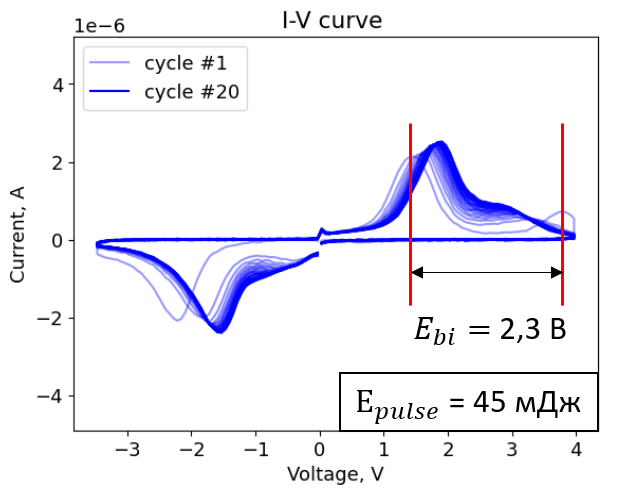
\includegraphics[width=0.49\linewidth]{probe_station/pq_45mJ.png}}
        \hfill
        \subcaptionbox{\label{fig:probe_station:pq_225mJ} Энергия импульса 225 мДж}{%
            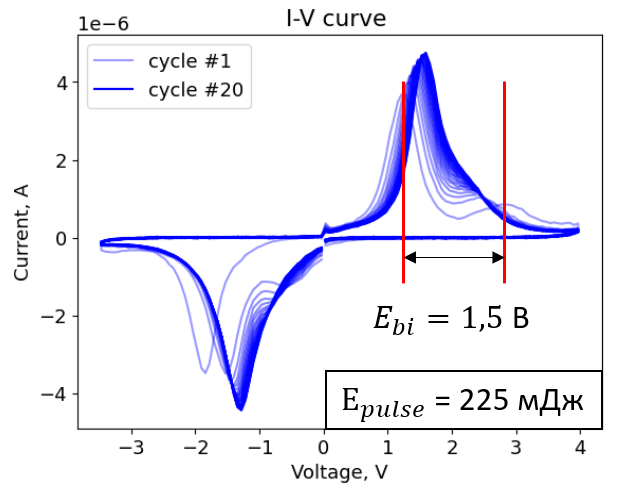
\includegraphics[width=0.49\linewidth]{probe_station/pq_225mJ.png}}
        \hfill
    }
    \caption[Этот текст попадает в названия рисунков в списке рисунков]{Вольт-амперных характеристики в процессе циклирования}\label{fig:probe_station:pq}
\end{figure}

% Одной из причиной образования внутренних полей является наличие градиента механических напряжений (флексоэлектрический эффект)





